

%\resizebox{0.98\textwidth}{!}{
	\begin{tabular}{c | c | c | c}
		\hline
		\thead{\footnotesize Class \\ \footnotesize Labels} & \thead{\footnotesize Natural \\ \footnotesize Images} & \thead{\footnotesize Iconic \\ \footnotesize Images} & \thead{\footnotesize Text \\ \footnotesize Descriptions} \\
		\hline 
		\makecell{ \scriptsize Granny Smith \\[-1pt] \scriptsize (Apple)}
		&  \makecell{ \begin{tikzpicture}
				\begin{scope}
					\node {\fbox{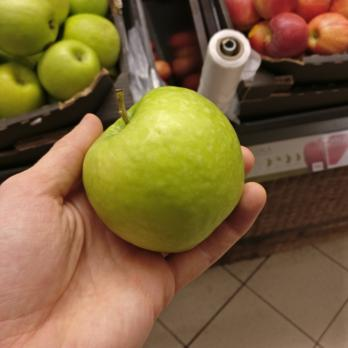
\includegraphics[width=30pt]{Chapter1/pics_paperA/Granny-Smith_021.jpg}}};
				\end{scope}
				\begin{scope}[xshift=34pt]
					\node {\fbox{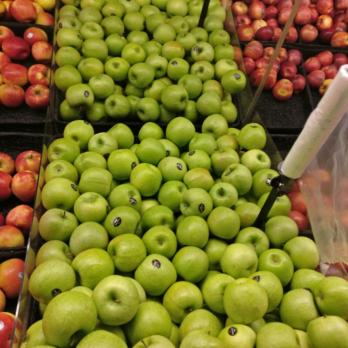
\includegraphics[width=30pt]{Chapter1/pics_paperA/Granny-Smith_012.jpg}}};
				\end{scope}
		\end{tikzpicture} }& 
		\makecell{\begin{tikzpicture}
				\begin{scope}
					\node {\fbox{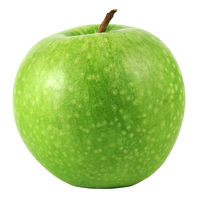
\includegraphics[width=30pt]{Chapter1/pics_paperA/Granny-Smith_Iconic.jpg}}};
				\end{scope}
		\end{tikzpicture} } & 
		\begin{scriptsize}
			\makecell{ \textit{“...\textbf{green} apple with \textbf{white, firm} pulp } \\[-1pt]  \textit{and a \textbf{clear acidity} in the flavor.”} } 
		\end{scriptsize}
		\\
		\hline 
		\makecell{ \scriptsize Tropicana \\[-1pt] \scriptsize Mandarin \\[-1pt] \scriptsize (Juice)}
		&  \makecell{ \begin{tikzpicture}
				\begin{scope}
					\node {\fbox{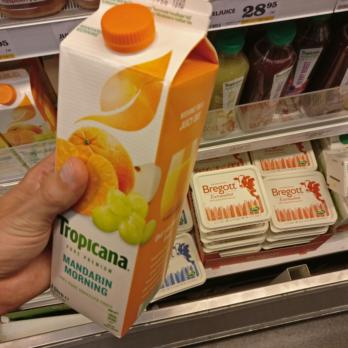
\includegraphics[width=30pt]{Chapter1/pics_paperA/Tropicana-Mandarin-Morning_003.jpg}}};
				\end{scope}
				\begin{scope}[xshift=34pt]
					\node {\fbox{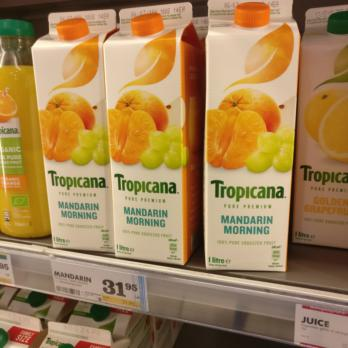
\includegraphics[width=30pt]{Chapter1/pics_paperA/Tropicana-Mandarin-Morning_016.jpg}}};
				\end{scope}
		\end{tikzpicture} }& 
		\makecell{\begin{tikzpicture}
				\begin{scope}
					\node {\fbox{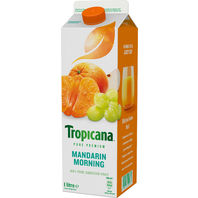
\includegraphics[width=30pt]{Chapter1/pics_paperA/Tropicana-Mandarin-Morning_Iconic.jpg}}};
				\end{scope}
		\end{tikzpicture} } & 
		\begin{scriptsize}
			\makecell{ \textit{“…is a \textbf{ready to drink} juice} \\[-1pt]
				\textit{\textbf{without pulp} pressed on \textbf{orange},} \\[-1pt]
				\textit{ \textbf{mandarin} and \textbf{grapes}. Not from} \\[-1pt]
				\textit{concentrate. Mildly \textbf{pasteurized}.” } }
		\end{scriptsize}
		\\
		\hline
	\end{tabular}
	%}